%%%%%%%%%%%%%%%%%%%%%%%%%%%%%%%%%%%%%%%%%%%%%%%%%%%%%%%%%%%%%%%%%%%%%%%%%%%%%%%%%%
\begin{frame}[fragile]\frametitle{}
\begin{center}
{\Large Calculus}
\end{center}
\end{frame}

%%%%%%%%%%%%%%%%%%%%%%%%%%%%%%%%%%%%%%%%%%%%%%%%%%%%%%%%%%%
 \begin{frame}[fragile]\frametitle{}
\begin{itemize}
\item Algebra deals with finite processes.
\item Calculus deals with infinitesimal processes.
\item Limiting situations.
\item Computers can not handle, need to approximate.
\end{itemize}
\end{frame}



%%%%%%%%%%%%%%%%%%%%%%%%%%%%%%%%%%%%%%%%%%%%%%%%%%%%%%%%%%%
 \begin{frame}[fragile]\frametitle{Main parts of Calculus}
\begin{itemize}
\item Numbers: how the number-line (`x' axis for single variable) is constructed. Various sets with infinite items.
\item Functions: Functions that generate numbers, their types.
\item Most real-life sets are finite, e.g. number of people in the world, number of hair on head, etc.
\item But numbers are infinite.
\end{itemize}
\end{frame}

%%%%%%%%%%%%%%%%%%%%%%%%%%%%%%%%%%%%%%%%%%%%%%%%%%%%%%%%%%%
 \begin{frame}[fragile]\frametitle{Basic Idea}
\begin{itemize}
\item Approximate/Divide
\item Compose the total
\item Reduce approximation infinitesimally small
\item Get the actual results
\end{itemize}
\end{frame}

%%%%%%%%%%%%%%%%%%%%%%%%%%%%%%%%%%%%%%%%%%%%%%%%%%%%%%%%%%%
 \begin{frame}[fragile]\frametitle{Basic Idea: Example}
\begin{itemize}
\item We know, circumference of circle is $2\pi r$
\item Whats the equation of area?
\end{itemize}
\end{frame}

%%%%%%%%%%%%%%%%%%%%%%%%%%%%%%%%%%%%%%%%%%%%%%%%%%%%%%%%%%%
 \begin{frame}[fragile]\frametitle{Basic Idea: Example}
Divide the circle into concentric strips, of $small$ widths.

\begin{center}
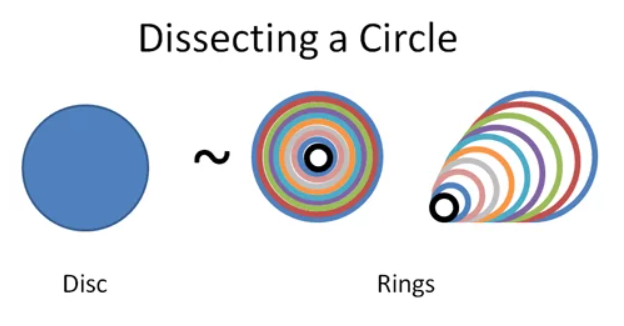
\includegraphics[width=0.7\linewidth,keepaspectratio]{calc1}
\end{center}

\tiny{(Ref: Lesson 1: 1 Minute Calculus: X-Ray and Time-Lapse Vision - Better Explained)}
\end{frame}

%%%%%%%%%%%%%%%%%%%%%%%%%%%%%%%%%%%%%%%%%%%%%%%%%%%%%%%%%%%
 \begin{frame}[fragile]\frametitle{Basic Idea: Example}
Compose to get the desired Area
\begin{center}
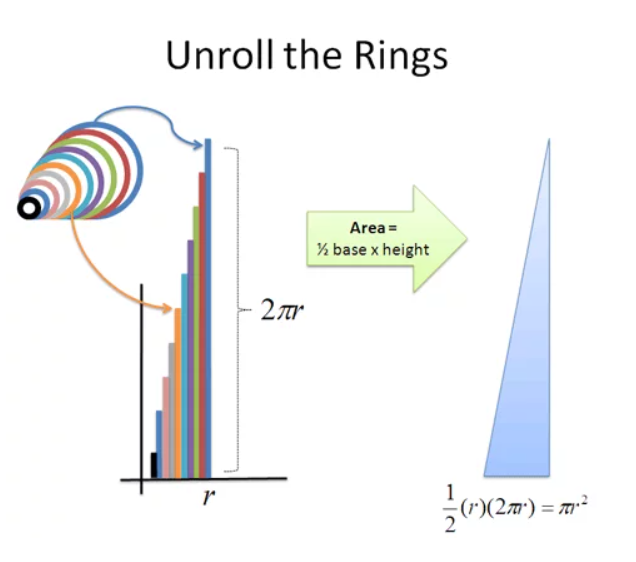
\includegraphics[width=0.65\linewidth,keepaspectratio]{calc2}
\end{center}

\tiny{(Ref: Lesson 1: 1 Minute Calculus: X-Ray and Time-Lapse Vision - Better Explained)}
\end{frame}

%%%%%%%%%%%%%%%%%%%%%%%%%%%%%%%%%%%%%%%%%%%%%%%%%%%%%%%%%%%
 \begin{frame}[fragile]\frametitle{Basic Idea: Example}

\begin{itemize}
\item Still approximate, right?
\item Reduce the approximation ie width to `infinitesimally' small to get accurate results.
\item This is called as \ldots ??
\end{itemize}

\tiny{(Ref: Lesson 1: 1 Minute Calculus: X-Ray and Time-Lapse Vision - Better Explained)}
\end{frame}

%%%%%%%%%%%%%%%%%%%%%%%%%%%%%%%%%%%%%%%%%%%%%%%%%%%%%%%%%%%
 \begin{frame}[fragile]\frametitle{Basic Idea: Example}
 
\begin{center}
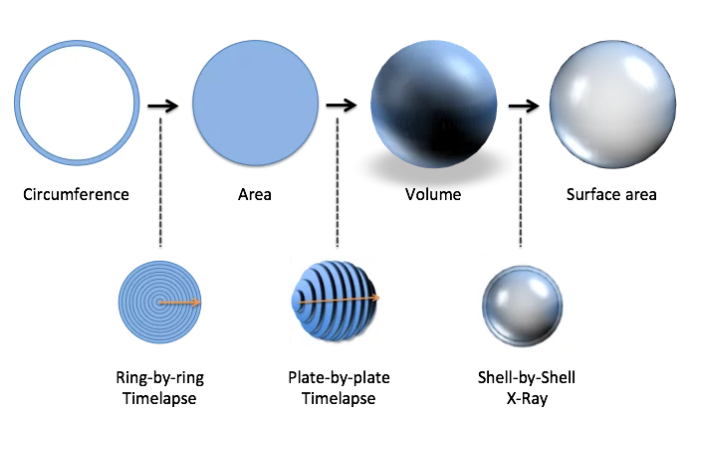
\includegraphics[width=0.7\linewidth,keepaspectratio]{calc3}
\end{center}


\begin{itemize}
\item Circumference with widths giving Area
\item Area slices with widths giving Volume
\item Slice places widths composed to give Surface Area
\end{itemize}

\tiny{(Ref: Lesson 3: Expanding Our Intuition - Better Explained)}
\end{frame}

%%%%%%%%%%%%%%%%%%%%%%%%%%%%%%%%%%%%%%%%%%%%%%%%%%%%%%%%%%%
 \begin{frame}[fragile]\frametitle{Basic Idea: Mathematical Notations}
 
\begin{center}
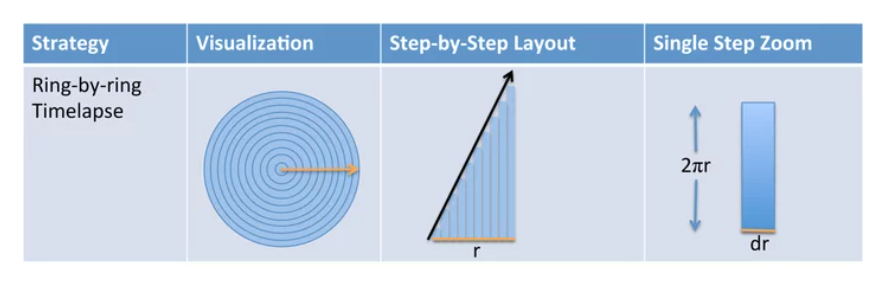
\includegraphics[width=0.7\linewidth,keepaspectratio]{calc4}
\end{center}

\tiny{(Ref: Lesson 4: Learning The Official Terms - Better Explained)}
\end{frame}

%%%%%%%%%%%%%%%%%%%%%%%%%%%%%%%%%%%%%%%%%%%%%%%%%%%%%%%%%%%
 \begin{frame}[fragile]\frametitle{Basic Idea: Mathematical Notations}
 
\begin{center}
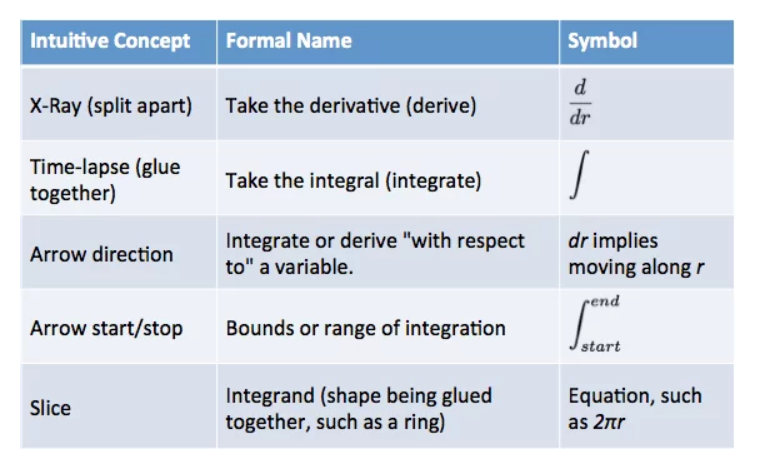
\includegraphics[width=0.9\linewidth,keepaspectratio]{calc5}
\end{center}

\tiny{(Ref: Lesson 4: Learning The Official Terms - Better Explained)}
\end{frame}

%%%%%%%%%%%%%%%%%%%%%%%%%%%%%%%%%%%%%%%%%%%%%%%%%%%%%%%%%%%
 \begin{frame}[fragile]\frametitle{Basic Idea: Algebra vs Calculus}
 
\begin{center}
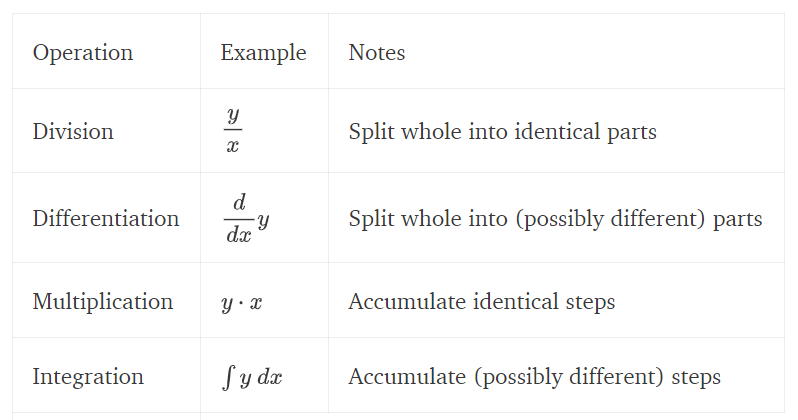
\includegraphics[width=0.9\linewidth,keepaspectratio]{calc6}
\end{center}

\tiny{(Ref: Lesson 6: Improving Arithmetic And Algebra - Better Explained)}
\end{frame}

%%%%%%%%%%%%%%%%%%%%%%%%%%%%%%%%%%%%%%%%%%%%%%%%%%%%%%%%%%%
 \begin{frame}[fragile]\frametitle{Basic Idea: More Formulas}
 
\begin{center}
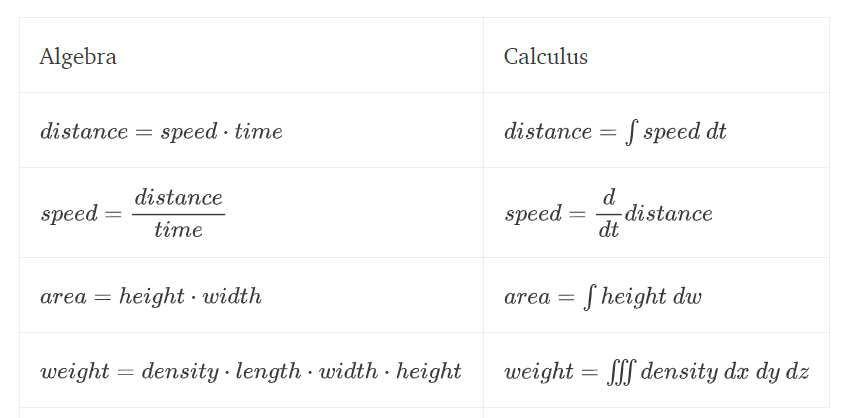
\includegraphics[width=0.9\linewidth,keepaspectratio]{calc7}
\end{center}

\tiny{(Ref: Lesson 6: Improving Arithmetic And Algebra - Better Explained)}
\end{frame}